\Chapter{Simulations}  
%%%%%%%%%%%%%%%%%%%%%%%%%%%%%%%%%%%%%%%%%%%%%%%%%%%%%%%%%%%%%%%%%%%%%%%%%%%%%%%%
%%%%%%%%%%%%%%%%%%%%%%%%%%%%%%%%%%%%%%%%%%%%%%%%%%%%%%%%%%%%%%%%%%%%%%%%%%%%%%%%
\Section{\lsnote{Introduction \sout{Code and Resources Used}}}\label{sec:code}
%%%%%%%%%%%%%%%%%%%%%%%%%%%%%%%%%%%%%%%%%%%%%%%%%%%%%%%%%%%%%%%%%%%%%%%%%%%%%%%%
%%%%%%%%%%%%%%%%%%%%%%%%%%%%%%%%%%%%%%%%%%%%%%%%%%%%%%%%%%%%%%%%%%%%%%%%%%%%%%%%

\lsnote{You need to start the chapter with summary paragraphs.  (1) Why are simulations needed?  (2) What simulation work was done?  (3) What method was chosen and why?  (4) What were the results?  You can't put  all of that in now, since some of it is unknown, but you should do (1), (3) and part of (2).  Also, before launching into the OPAL stuff, you need to say a few words about the beam characteristics during TBA studies.  A table of beam characteristics would be good here, one for the drive beam, and one for the witness.  After presenting the beam characteristics, you can mention that space charge is a problem for the drive beam - since now they know the intensity.}

With  the  rapid  improvement  in  computing  resources  and  codes  in  recent  years,  
accelerator  facilities  can  now achieve and rely on accurate beam dynamics simulations. 
These  simulations  include  single  particle  effects  (e.g. particle tracking in a magnetic field) as well as collective effects  such  as  space  charge  (SC),  
and  coherent  synchrotron  radiation  (CSR).

The beam dynamics reported in this thesis, were simulated with 
the open source, particle-in-cell (PIC) code OPAL \lsnote{\sout{was used}} \cite{opal}. 
PIC codes simulate the electromagnetic forces that particles see in an accelerator. 
This is done by mapping the input particles onto a grid. 
Then in each time (or z) step, the forces due to space charge, accelerating gradients, 
and magnets are calculated and applied to the grid.
OPAL comes in two flavors, OPAL-CYC and OPAL-T. The first is used to model 
cyclotrons, and the latter, which is used for this work, is suited for photoinjectors. 
OPAL-T was chosen in part because it models the 3D space charge necessary to accurately simulate the high charge bunches at the AWA. 
It was chosen for several reasons:
\begin{itemize}
	\item Able to calculate transverse space charge and wakefield forces 
	\item Option to run the code in parallel
	\item Data recorded in global and reference frames \lsnote{did you mean `and local reference frames'?}
\end{itemize} 

The first item is crucial to standard operations at the AWA. Especially in the 
case of TBA, high charge is needed on drive beam line, therefore transverse 
space charge must be calculated in the simulations to give realistic results.
The second item dramatically reduced the amount of simulation time needed. 
For example, simulating the gun and linac, about \SI{15}{m} of elements,
with 100,000 particles on one core would take about 30 minutes. 
When the number of cores is increased to 16, the same run takes less than 
5 minutes. This reduction in time by ~80\%, combined with the capability to run 
many cases at once on the cluster allows for more efficient use of time.
Typical running conditions were on 16 cores, for random samples up to 128 cores, 
and up to 5,200 cores for large optimization runs.  


%%%%%%%%%%%%%%%%%%%%%%%%%%%%%%%%%%%%%%%%%%%%%%%%%%%%%%%%%%%%%%%%%%%%%%%%%%%%%%%%
%%%%%%%%%%%%%%%%%%%%%%%%%%%%%%%%%%%%%%%%%%%%%%%%%%%%%%%%%%%%%%%%%%%%%%%%%%%%%%%%
\Section{Benchmarking}

\nrnote{Copied and pasted NAPAC benchmark here, need to finish cleaning up.}
\lsnote{ {\it Suggestion if accurate:} Initially OPAL-T was benchmarked against the more established particle tracking codes, ASTRA and GPT.  This ensured correct use of the code, and reliability of \mbox{OPAL-T}.  Two collective effects of particular interest to the AWA were included in the investigation: 
space charge (SC) and coherent synchrotron radiation (CSR).
\sout{Using portions of AWA as the benchmark model,  
beam dynamics were simulated with three particle tracking codes.
The AWA rf photoinjector was benchmarked, primarily to study SC, 
in ASTRA, GPT, and OPAL-T using}  The beam dynamics of a \SI{1}{nC} drive beam in the photoinjector were used as the model for comparison in the space charge study.} A $20^{\circ}$ hard edge dipole magnet was used to benchmark CSR effects in GPT and OPAL-T by bending a 1nC beam 
at  energies  between  2  MeV  and  100  MeV.  \lsnote{The results of these benchmark studies are presented below, including a discussion of  \sout{In  this  paper  
we  present  the  results,  and  discuss}}  the  similarities  and  
differences between the codes.
 
The AWA group has used several beam codes in the past including:
T-STEP/PARMELA~\cite{parmela}, ASTRA~\cite{astra}, and GPT~\cite{gpt}.  
In order to take advantage of computing resources offered by 
Argonne National Laboratory (ANL), \lsnote{an investigation of \sout{effort was made to investigate}}
OPAL~\cite{opal} \lsnote{was done; this is} an open source and parallel code that comes in two flavors;  
OPAL-CYL and OPAL-T. The latter was installed on the Blues and Bebop \lsnote{high performance computing} clusters
at the Laboratory Computing Resource Center (LCRC) provided by ANL~\cite{lcrc}.
(See Appendix~\ref{build} for instruction on how to build OPAL-T at ANL.)

\lsnote{{\it I combined this in the modified first paragraph:}\sout{Since no members of AWA had prior experience with OPAL-T, a benchmark 
was done to compare \mbox{OPAL-T} results to the results of codes 
well known to the group (GPT and ASTRA). 
This ensured correct use of the code, and reliability of \mbox{OPAL-T}.
Two collective effects of interest to the AWA were used: 
space charge (SC) and coherent synchrotron radiation (CSR).
SC was tested using the drive gun at 1nC, and CSR was tested
using a hard edge dipole.}}


\Subsection{Gun Simulations}
The SC algorithms were probed using the AWA photoinjector, 
a 1.5 cell copper standing-wave cavity at 1.3 GHz, 
with bucking, focusing, and matching solenoids. 
In the remainder of this thesis, the word gun is used 
in place of photoinjector. The simulation parameters were chosen to 
approximately generate the canonical “\SI{1}{\micro\metre} at 1 nC” case.  \lsnote{These values refer to the 2D transverse emittance and the bunch charge.  {\it correct?}}
The initial beam parameters were based on gun operations at PITZ \cite{pitz},
due to the similarities between the PITZ and AWA rf guns.
The PITZ parameters came close to achieving the \SI{1}{\micro\metre}
target without any optimization. A coarse 1D minimization
\nrnote{add method used here} of the 
emittance was done to determine the value of the laser radius 
used in this benchmark. The resulting minimum emittance was   
\SI{1.16}{\micro\metre}. 

The initial bunch distribution parameters as well as the 
on-axis gun gradient, and magnetic field \lsnote{of the solenoids} used in 
the benchmark are listed in Table~\ref{tab:bench}. 
The rf gun and solenoid field maps were generated 
with the SUPERFISH/POISSON  codes~\cite{superfish}.
The gradient was chosen to match typical operations at PITZ~\cite{pitz}
and the AWA. The rf and solenoid fields seen by the beam in the gun are shown in Fig.~\ref{fig:gunfields}.
\begin{table}
	\begin{center}
		\begin{tabular}{l l} 
			\toprule
			\textbf{Parameter} & \textbf{Value} \\ 
			\midrule
			Charge & \SI{1}{nC} \\
			\addlinespace[-1em] 
			Gradient & \SI{60}{MV/m} \\
			\addlinespace[-1em] 
			Phase & Max energy (on crest) \\
			\addlinespace[-1em] 
			Laser radius & \SI{0.75}{mm} \\
			\addlinespace[-1em] 
			Rise and fall time & \SI{6}{ps} \\
			\addlinespace[-1em] 
			Initial kinetic energy & \SI{0.55}{eV} \\
			\addlinespace[-1em] 
			Matching solenoid strength & \SI{-0.389}{T} \\
			\addlinespace[-1em] 
			Buck and focusing solenoid strength & \SI{-0.12}{T} \\
			\bottomrule			
		\end{tabular}
	\end{center}
	\caption{Input simulation parameters for gun benchmark.}
\end{table}\label{tab:bench}
\begin{figure}
	\begin{center}
		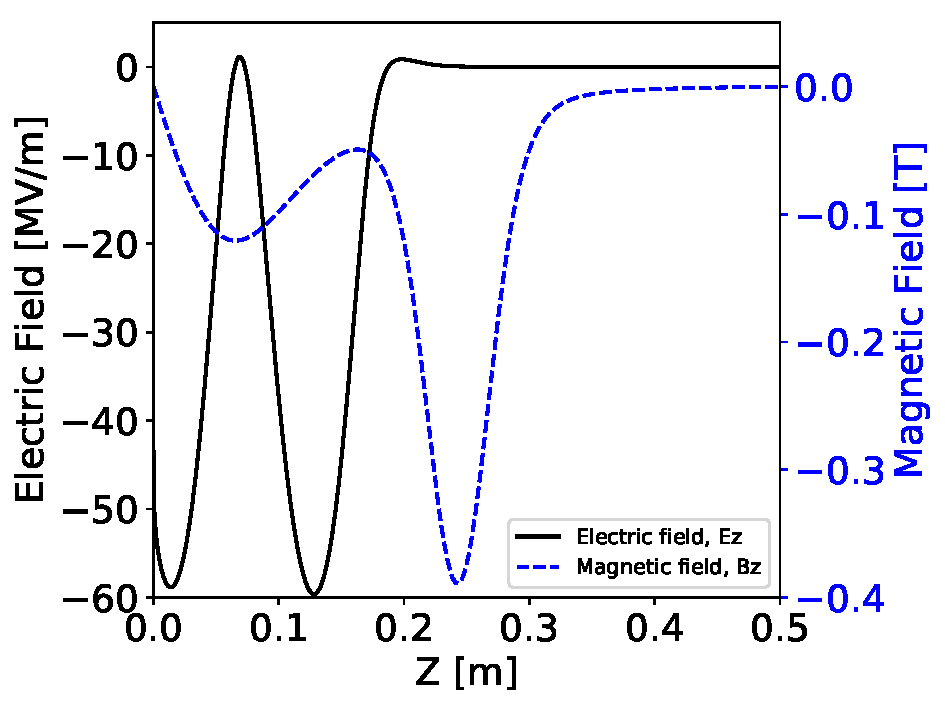
\includegraphics[width=0.95\textwidth]{images/gun_EM_fields}\caption{Electric and magnetic fields seen by the beam on axis in the gun.  \lsnote{Specify the Z distance to end of gun in figure caption}}
	\end{center}
\end{figure}\label{fig:gunfields}

\lsnote{the figure number for the gun fields doesn't match the reference}\\
Note that the codes use various methods to model 
the rf and magnetic fields, SC, and image charge. 
The ASTRA simulations used the axial E field of the  
gun and solenoids, and then \lsnote{extended \sout{expanded}} the fields to find the
transverse components using the paraxial approximation 
(e.g. $E_r=-\frac{r}{2}\frac{dE_z}{dz}$). 
The \lsnote{simulation  \sout{s}} used a 2D cylindrical-symmetric SC algorithm with a uniform  
particle-deposition mesh; see ASTRA user manual~\cite{astra}.
The radial and longitudinal number of cells composing the mesh 
were $N_r=32$ and $N_z=64$, with 100k particles.  
The image charge close to the cathode was accounted for until 
the bunch reached \SI{9.7}{cm} from the cathode surface. 

GPT read in the 2D electric and magnetic field files,  
and used a square 3D adaptive SC mesh with $N_x=N_y=N_z=46$
with 100k particles, see spacecharge3Dmesh option in GPT manual~\cite{gpt}.
To calculate image charge, GPT uses a Dirichlet boundary condition at the  
cathode (z=0). The calculation is turned off when the  
distance between the beam and cathode is longer than the 
mesh box. OPAL-T also read in the field maps, and used a block 
structured equidistant SC mesh, see OPAL manual for SC calculation~\cite{opal}.  
Several square mesh sizes were run in OPAL-T. The results plotted in 
Fig.~\ref{fig:benchplot_gun} and~\ref{fig:benchplot_5m} correspond to a mesh of $N_x=N_y=N_z=46$, with 1 million particles. 
The image charge calculation uses a 
shifted integrated Green function \cite{imagecharge}.  
\begin{figure}
	\begin{center}
		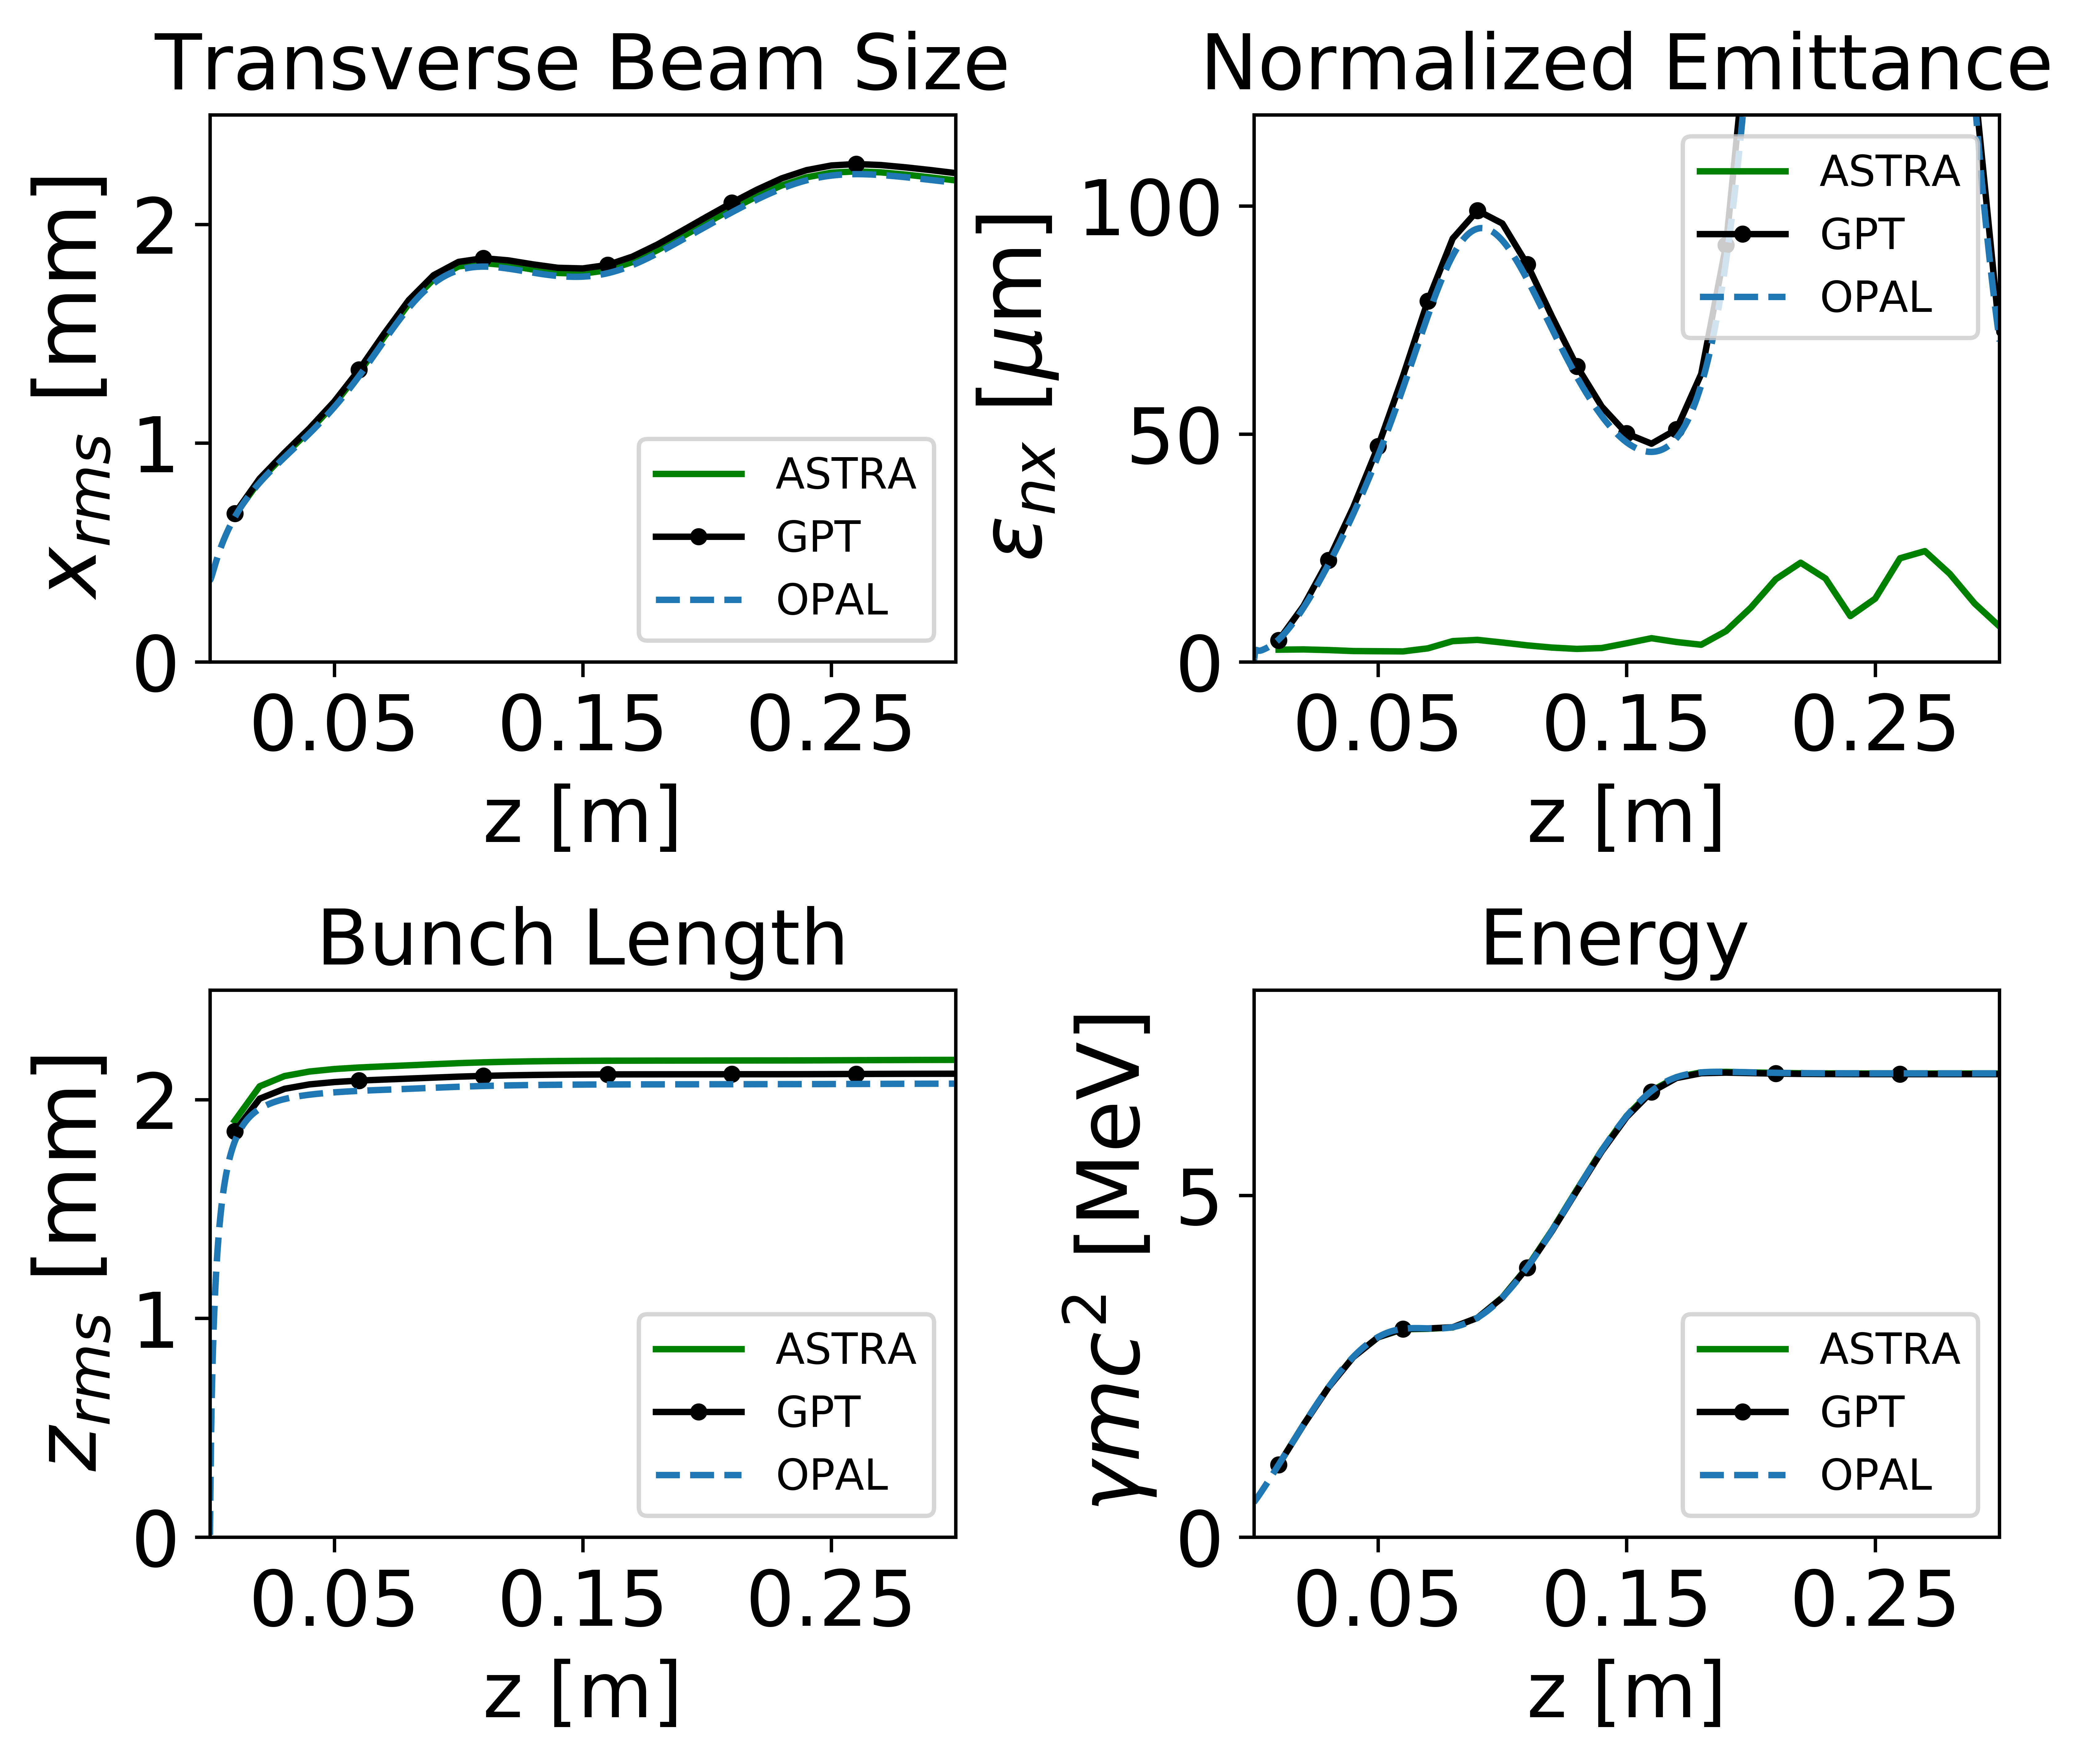
\includegraphics[width=0.8\textwidth]{images/benchmark_gun}
		\caption{Beam envelopes in the gun.}
	    \label{fig:benchplot_gun}

        \vspace*{\floatsep}
        
		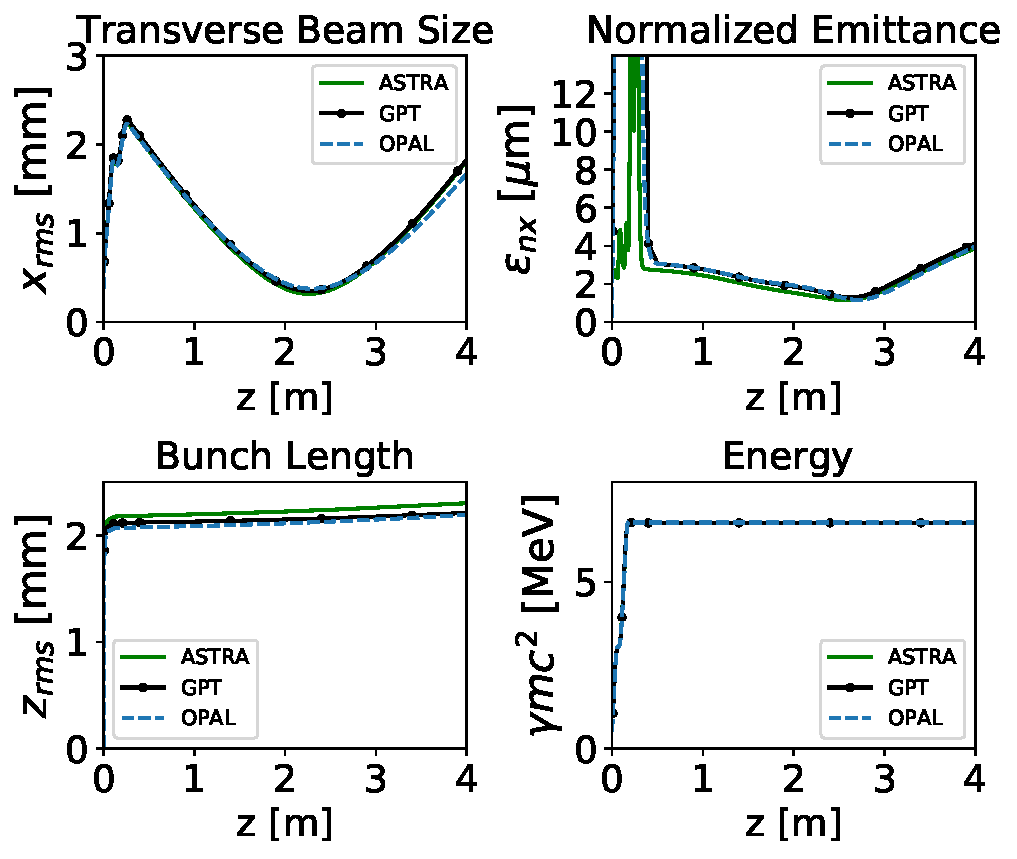
\includegraphics[width=0.8\textwidth]{images/benchmark_5m}
		\caption{Beam envelopes in drift.}
	    \label{fig:benchplot_5m}
	\end{center}
\end{figure}

In general, the simulation results are in reasonable agreement 
and within expectations based on previous benchmarks \cite{codecompare}. 
See Figs.~\ref{fig:benchplot_gun} and~\ref{fig:benchplot_5m} 
for \lsnote{a comparison of the} beam envelopes \lsnote{generated by the three simulations} in the gun and drift. 
The apparent disagreement of emittance between ASTRA and the other
two codes in the gun is because the former removes the angular momentum   
induced by the solenoid, while the \lsnote{other \sout{later}} two codes do not. 
After the beam exits the solenoid, the emittance results  
are in good agreement, as shown in Fig.~\ref{fig:benchplot_5m}.

\Subsection{Dipole \lsnote{Simulations}}
Simulations  of  a  hard  edge  dipole  were  done  in  GPT  
and   OPAL-T   in   order   to   probe   \lsnote{the} CSR \lsnote{results}.   Short   
mono-energetic  \lsnote{Bunches with a Gaussian  energy distribution \sout{Gaussian bunches}}  with  zero  initial \lsnote{transverse} emittance  
were sent through the dipole. \lsnote{{\it If Gaussian in transverse parameter cannot be `zero emmittance'}} Beam and dipole parameters 
are shown in Table~\ref{tab:benchcsr}. \lsnote{weird table number}
The CSR routine used in OPAL-T is based on 
the routine  used  in  ELEGANT  \cite{elegant}, which is known to assume  
the beam is ultra-relativistic. The CSR routine in GPT  
does  not  use  the  ultra-relativistic  approximation ($\beta=1$) 
and  as  a  result,  works  at  all energies  \cite{gptcsr}.  
Therefore, we expected  the  routines  to  match  well  at  high  energy  and  
diverge  at  lower  energy.  Results  of  the  CSR  simulations  
are  shown  in  Fig.  4.  \lsnote{{\it missing figure}} As  expected,  the  results  between  
GPT and OPAL-T disagree at low energies. 
\begin{table}
	\begin{center}
		\begin{tabular}{l l} 
			\toprule
			\textbf{Parameter} & \textbf{Value} \\ 
			\midrule
			$\sigma_x =\sigma_y$ & \SI{1}{mm} \\
			\addlinespace[-1em] 
			Gradient & \SI{60}{MV/m} \\
			\addlinespace[-1em] 
			Phase & Max energy (on crest) \\
			\addlinespace[-1em] 
			Laser radius & \SI{0.75}{mm} \\
			\addlinespace[-1em] 
			Rise and fall time & \SI{6}{ps} \\
			\addlinespace[-1em] 
			Initial kinetic energy & \SI{0.55}{eV} \\
			\addlinespace[-1em] 
			Matching solenoid strength & \SI{-0.389}{T} \\
			\addlinespace[-1em] 
			Buck and focusing solenoid strength & \SI{-0.12}{T} \\
			\bottomrule			
		\end{tabular}
	\end{center}
	\caption{Input simulation parameters for gun benchmark.}
\end{table}\label{tab:benchcsr}


\Subsection{Convergence Study}
\lsnote{Did you do these convergence runs for all three codes?  If yes, some comparison to other codes needed.  If not, this does not belong in the benchmark section.  In that case, you need to move your `benchmark conclusion' before this paragraph.  Also, then you need to wrap up this paragraph with a concluding sentence or two.  It can be its own section, even though short.}
Convergence runs were done for three parameters: 
time step,  SC  mesh  size,  and  number  of  particles.  
Each  case was tested in the gun using the same field maps and 
baseline  settings  that  were  used  to  compare  SC  in  OPAL-T,  
ASTRA, and GPT. All OPAL-T simulations were run on 
16 cores, taking advantage of parallel calculations. 
The number of particles was varied from 20k to 3.2  million.  
The  longitudinal  parameters  (energy,  bunch length)  
showed  no  variation,  but  there  were  slight  deviations 
in the transverse emittance and beam size. The same results 
were observed when the time step was varied from 0.1 ps  to  10  ps.  
The  grid  size  was  changed  from  32,  44,  46, and 64 cubed; 
again the results lacked any major discrepancies.  
In all cases, no appreciable differences were observed in the energy,
emittance, beam size, or bunch length. In  most  cases,  
if unreasonable  parameters  were chosen, 
OPAL-T would not complete the run (crash or hang up).  

\nrnote{conclusion}
Based on the experience gained during this benchmark, 
all  three  codes  are  capable  of  accurate  simulations.  With  
respect  to  resources  at  the  AWA:  GPT  and  ASTRA  are  
better  suited  for  use  on  windows,  and  OPAL-T  is  better  
suited to Linux and parallel systems.

%At 40nC the usable gun phase range (for the 3D field map) is 
%$-30^\circ \le \phi_g \ge 30^\circ$. The usable region was defined 
%as the region where all particles are emitted from the gun. 
%i.e. at $40^\circ$, particles were lost. 
%%%%%%%%%%%%%%%%%%%%%%%%%%%%%%%%%%%%%%%%%%%%%%%%%%%%%%%%%%%%%%%%%%%%%%%%%%%%%%%%
%%%%%%%%%%%%%%%%%%%%%%%%%%%%%%%%%%%%%%%%%%%%%%%%%%%%%%%%%%%%%%%%%%%%%%%%%%%%%%%%
\Section{Optimization} \label{sec:opt}
Throughout the design process, optimization algorithms 
were used to \lsnote{\sout{shape} study} the beam \lsnote{parameters at the entrance of \sout{entering}} the TBA experimental area.
Minimizing the emittance and bunch length after the six cavity linac,
and choosing the optimal optics configuration for maximum beam transport 
were the main objectives of all optimization work.
The techniques used include model based, genetic,
and structure exploiting algorithms. 
 
Model-based, derivative-free, trust-region algorithms 
are increasingly popular for optimizing computationally 
expensive numerical simulations. \lsnote{Not being an expert, I personally would like to see a quick 
definition of `model-based', `derivative-free, and `trust-region'.  This helps the general reader to 
better track what you are doing.}  A strength of such
methods is their efficient use of function evaluations. 
\lsnote{\sout{This was the first type of algorithm used to optimize 
the beam dynamics in two cases of interest at the AWA.}}  

\lsnote{{\it There is an organizational problem here.}  You need to finish the `introduction' before launching into specifics.  The two paragraphs after the following one seem like part of the intro, you say why you used the genetic algorithm, and then how you reduced the time.  This goes with the overall picture of the intro.  You also need to give a {\it brief} explanation of what genetic algorithms and structure based agorithms are (as well as model-based) in the intro.  Then you can have a new subsection; `model-based algorithm studies' before launching into the following paragraph.}

The model-based algorithm was the first type of algorithm used to optimized the beam dynamics in two cases of interest at the AWA.  \lsnote{The first case was for lower beam charge, and used only the gun parameters for the optimization.  The second case was for higher beam charge, and included parameters of the downstream linac as well as the gun.} 
\lsnote{In the first case, \sout{First,}} the emittance of a \SI{1}{nC} electron 
bunch produced by the AWA rf photocathode gun 
was minimized by adjusting three parameters: rf gun phase, 
solenoid strength, and laser radius. The algorithm 
\lsnote{converged} to a set of parameters that \lsnote{yielded} an
emittance of \SI{1.08}{\um}. \lsnote{In the second case, \sout{Second, we expand}} 
the number of optimization parameters \lsnote{was expanded} to model the complete AWA rf 
photoinjector (the gun and six accelerating cavities) at \SI{40}{nC}. 
The optimization algorithm was used in a Pareto \lsnote{study; which is a type of study} that compares the 
trade-off between \lsnote{competing parameters, such as} emittance and bunch 
length \lsnote{at the exit of \sout{for}} the AWA \SI{70}{MeV} photoinjector. \nrnote{finished?}

\lsnote{Following two paragraphs should be part of intro.  Then the details in separate sub-sections.}
After a model based method was implemented, a common technique was 
used as confirmation and for exploratory work. Preliminary designs 
for the TBA optics configuration were probed using a Genetic Algorithm
that was built in to OPAL.  \nrnote{running simulations now}

Finally, to reduce the amount of time needed to optimize the complete beam line, 
a structure exploiting algorithm was implemented. \nrnote{working on this}


\Subsection{Bounded Optimization by Quadratic Approximation (BOBYQA)}
%\section{Optimization Algorithm}
% ----------------------------------------------------
Model-based, derivative-free algorithms are frequently used to optimize
computationally expensive simulations due to their judicious use of function
evaluations. In cases specific to accelerator physics, 
beam properties at different operational parameters are observed;
these methods then build models of the unknown
function and minimize these models to identify candidate parameters to 
evaluate. BOBYQA~\cite{bobyqa} is one such method that is available via the
NLopt~\cite{nlopt} package and was used in this study. 
Given a candidate set of optimal parameters $v^k$, BOBYQA
constructs a quadratic model using function values of points near $v^k$. 
This model is minimized in a neighborhood of $v^k$ in order to produce a point $\hat{v}$. If $\hat{v}$ has a smaller objective function value than $v^k$, 
the estimate of the optimum is updated to $\hat{v}$, and a new model is constructed. 
If $\hat{v}$ is not a sufficient improvement over $v^k$, 
the model around $v^k$ is improved. For more
information about derivative-free optimization, see~\cite{Conn2009a}.

The parameters $v^k$ are generated and supplied to OPAL\=/T~\cite{opal}. 
The optimization package NLopt and OPAL\=/t were used
in combination with Python code written at ANL with the help 
of Jeff Larson, to perform simulation evaluations and optimization.
All the files needed to replicate the results in this section are available \lsnote{at: $<$www.mcs.anl.gov/$\sim$jlarson/AWA$>$.  {\it Put previous on same line of text, then delete below until the next subsection.}}

\begin{center}
	www.mcs.anl.gov/$\sim$jlarson/AWA
\end{center}

\lsnote{\sout{Interested parties are welcome to adapt the code to their needs
and suggest improvements.}}

\Subsection{Optimization Parameters}
% ----------------------------------------------------
When optimizing the gun, three parameters \lsnote{$v^k$ {\it (add to better tie to previous paragraph)}} were varied: 
solenoid strength ($S_3$), gun phase ($\phi_g$), 
and laser radius ($R$) of a uniform \lsnote{ photon distribution \sout{pulse}}. 
The minimized objective was emittance ($\epsilon_x$).
(The \lsnote{reference} phase \lsnote{of the gun} is defined as $0^{\circ}$ at maximum \lsnote{accelerating voltage \sout{energy gain}}.) 
When optimizing the \lsnote{gun and the} entire linac, seven additional parameters were 
varied: the longitudinal \lsnote{duration of the} laser \lsnote{pulse, defined at} full width at half maximum ($T$)
and accelerating cavity phases ($\phi_L$). The optimization parameters and
bounds are given in table~\ref{tab:parameters}; we denote the set of
ten optimization parameters as $v=[S_3, \phi_g, R, T, \phi_L]$, where 
$\phi_L=[\phi_{L_1},\ldots,\phi_{L_6}]$ represents the phase of each linac cavity $L_1$-$L_6$. 
\nrnote{need to fix footnotes and superscripts for table 3.3}
\begin{table}
	\caption{\label{tab:parameters} Parameter bounds for gun and linac optimization.}
	\begin{center}
		\begin{tabular}{ l *{3}{c}} 
			\toprule
			\textbf{Variable} & \textbf{Range} & \textbf{Unit} \\
			\midrule
			Solenoid Strength & $ 0 \le S_3 \le 440$  & amps \\
			Phase of Gun & $-60 \le \phi_g \le 60$  & degrees \\
			Laser Radius  & $0.1 \le R \le 30$  & mm \\
			Laser FWHM \footnotemark \label{note1}& $2 \le T \le $10  & ps \\
			Cavity Phase \textsuperscript{\ref{note1},}\footnotemark & $-20 \le \phi_L \le 20$  & degrees \\
			\bottomrule	
		\end{tabular}
	\addtocounter{footnote}{-1}\footnotetext{not varied during gun optimization}
	\addtocounter{footnote}{+1}\footnotetext{$\phi_L=[\phi_{L_1},\ldots,\phi_{L_6}]$}
	\end{center}
\end{table}


\Subsection{Gun Simulations Using BOBYQA} \label{sec:gunbobyqa}
%\section{Gun Optimization}
% ----------------------------------------------------
\lsnote{There has been \sout{Much}} work \lsnote{\sout{has been}} done \lsnote{by other groups} to optimize 1.5 cell rf guns
at \SI{1}{nC}~\cite{pitz}. \lsnote{The \sout{This}} known solution \lsnote{from that work} was used as 
a baseline test of BOBYQA when applied to \lsnote{this \sout{an}} accelerator application.
An optimization of the single objective emittance ($\epsilon_x$) was 
performed over a length of \SI{5}{m}. 
All linacs were turned off and only gun parameters were varied. 
Non-varying parameters are listed in table~\ref{tab:gun}; 
their values are based on \lsnote{realistic parameters \sout{work done}} at PITZ and AWA~\cite{pitz, benchmark}.

Local optimization runs were started \lsnote{using \sout{from}} five points \lsnote{per parameter?  {\it If yes, add that here.}} with various \lsnote{differences \sout{distances}} from the optimum value. The optimization runs converged 
(in less than 100 function evaluations) to a parameter set ($S_3=\SI{269}{A}$, $\phi_g=\SI{-3.0}{^{\circ}}$, and $R=\SI{0.6}{mm}$) 
with an emittance of $\SI{1.08}{\um}$.
An exhaustive search of the parameter space was not done, and there may be other local minima that were not found.
However, the results match expectations based on the literature. 
\begin{table}[h] 
	\caption{\label{tab:gun} Non-varying parameters for gun optimization.}
	\begin{center}
		\begin{tabular}{lll}
			\toprule
			\textbf{Parameter} & \textbf{Value} \\
			\midrule
			Charge  & \SI{1}{nC} \\
			Gradient & \SI{60}{MV/m} \\
			Laser FWHM & \SI{20}{ps} \\
			Laser Rise and Fall Time & \SI{6}{ps} \\
			Kinetic Energy at Cathode  & \SI{0.55}{eV} \\
			$S_1$ and $S_2$ & \SI{550}{A} \\
			\bottomrule
		\end{tabular}
	\end{center}
\end{table}


\lsnote{I would not make below a subsection, I would keep the figure and put the information from the description below into the figure caption instead.  I tried to shorten it up a bit.}\\
\Subsection{Linac Description} \label{sec:pareto}
\nrnote{maybe this beam line description should be in chp 2:}\\
The \SI{70}{MeV} \lsnote{AWA} rf photoinjector \lsnote{\sout{at the AWA}}
\lsnote{is \sout{consists of}} an rf gun followed by \lsnote{a linac with} six rf accelerating cavities, 
\lsnote{ labeled $L_1$-$L_6$ \cite{Power:2010zza}.  The cavity phases are constrolled independently. \sout{hereafter referred to as the linac. 
See Figure~\ref{fig:beamline} for the beam line layout.} } 
The 1.5 cell rf gun operates at \SI{1.3}{GHz} with three solenoids 
and a Cs$_{2}$Te photocathode excited by a \SI{248}{nm} UV laser.  
Solenoid 1 ($S_1$) is used to buck the field at the cathode,
while the other two solenoids ($S_2$ and $S_3$) are used for emittance compensation.  
\lsnote{\sout{The accelerating cavities, also operated at  1.3 GHz are 7 cell standing-wave 
cavities \cite{Power:2010zza} each with independently controllable phase. The cavities are labeled
$L_1$-$L_6$ in Figure(fig:beamline). } }

\def \gunleft {-1.0}
\def \gunright {0.3}
\def \loneright {1.0}
\def \ltworight {3.5}
\def \lthreeright {5.0}
\def \lfourright {7.0}
\def \lfiveright {8.5}
\def \lsixright {10}
\begin{figure*}
	\captionsetup{width=0.98\linewidth}
	\begin{center}
		
		\begin{tikzpicture}[scale=0.95]
		%Gun drawings
		\draw[fill=orange, very thick, rounded corners =0.1cm] (\gunleft,0.5)rectangle (\gunright,1.5) node[pos=.5, white] {\textbf{Gun}} ;
		
		%S1
		\node[] at (-1.3,2.9) {$S_1$};
		\draw[ultra thick, fill=black!60!green] (-1.4,-0.5)rectangle  (-1.0,0.5) node[pos=.5, white] {} ;
		\draw[black, ultra thick] (-1.4,-0.5) -- (-1.0,0.5);
		\draw[black, ultra thick] (-1.4,0.5) -- (-1.0,-0.5);
		\draw[ultra thick, fill=black!60!green] (-1.4,1.5)rectangle  (-1.0,2.5) node[pos=.5, white] {} ;
		\draw[black, ultra thick] (-1.4,1.5) -- (-1.0,2.5);
		\draw[black, ultra thick] (-1.4,2.5) -- (-1.0,1.5);
		%S2
		\node[] at (-0.8,2.9) {$S_2$};
		\draw[ultra thick, fill=black!60!green] (-1.0,-0.5)rectangle  (-0.6,0.5) node[pos=.5, white] {} ;
		\draw[black, ultra thick] (-1.0,-0.5) -- (-0.6,0.5);
		\draw[black, ultra thick] (-1.0,0.5) -- (-0.6,-0.5);
		\draw[ultra thick, fill=black!60!green] (-1.0,1.5)rectangle  (-0.6,2.5) node[pos=.5, white] {} ;
		\draw[black, ultra thick] (-1.0,1.5) -- (-0.6,2.5);
		\draw[black, ultra thick] (-1.0,2.5) -- (-0.6,1.5);
		
		%S3
		\node[] at (0.2,2.9) {$S_3$};
		\draw[ultra thick, fill=black!60!green] (-0.1,-0.5) rectangle  (0.3,0.5) node[pos=.5, white] {};
		\draw[black, ultra thick] (-0.1,-0.5) -- (0.3,0.5);
		\draw[black, ultra thick] (-0.1,0.5) -- (0.3,-0.5);
		\draw[ultra thick, fill=black!60!green] (-0.1,1.5) rectangle  (0.3,2.5) node[pos=.5, white] {};
		\draw[black, ultra thick] (-0.1,1.5) -- (0.3,2.5);
		\draw[black, ultra thick] (-0.1,2.5) -- (0.3,1.5);
		%Linac drawings 
		\draw[fill=blue, ultra thick, rounded corners =0.1cm] (\loneright,0)rectangle  ({\loneright+0.84},2) node[pos=.5, white] {$L_1$} ;
		\draw[fill=blue, ultra thick, rounded corners =0.1cm] (\ltworight,0)rectangle  ({\ltworight+0.84},2) node[pos=.5, white] {$L_2$};
		\draw[fill=blue, ultra thick, rounded corners =0.1cm] (\lthreeright,0)rectangle ({\lthreeright+0.84},2) node[pos=.5, white] {$L_3$};
		\draw[fill=blue, ultra thick, rounded corners =0.1cm] (\lfourright,0)rectangle ({\lfourright+0.84},2) node[pos=.5, white] {$L_4$};
		\draw[fill=blue, ultra thick, rounded corners =0.1cm] (\lfiveright,0)rectangle ({\lfiveright+0.84},2) node[pos=.5, white] {$L_5$};
		\draw[fill=blue, ultra thick, rounded corners =0.1cm] (\lsixright,0)rectangle ({\lsixright+0.84},2) node[pos=.5, white] {$L_6$};
		\draw[very thick] (\gunleft,-1.5) -- (14,-1.5);
		\draw[latex-latex] (\gunleft,-1.5) -- (14,-1.5) ; 
		\foreach \x in  {0.3, 1.0, 3.5, 5.0, 7.0, 8.5, 10, 12.5} %tick marks
		\draw[shift={(\x,-1.5)},color=black] (0pt,3pt) -- (0pt,-3pt);
		\foreach \x in {0.3, 1.0, 3.5, 5.0, 7.0, 8.5, 10, 12.5}
		\draw[shift={(\x,-1.7)},color=black] (0pt,0pt) node[below] 
		{$\x$};
		
		\node[draw, fill=yellow, star, star points=5, star point ratio=0.6, minimum size=0.6cm]
		at (12.5,1.0) {$z_1$};
		\end{tikzpicture}
	\end{center}
	\caption{Layout of the AWA linac. \lsnote{You could insert your paragraph here, then delete what follows up until the sentence beginning with `Tick marks..'}
		The gun is enlarged to show solenoid detail. The physical length is
		\SI{0.3}{m}. The cathode is located at $z=\SI{0}{m}$. Linac cavities are
		\SI{0.85}{m} long. Tick marks are located at the exit of the gun, entrance of
		each accelerating cavity, and location of optimization.}
	\label{fig:beamline} 
\end{figure*} 

\Subsection{Linac Optimization}
%\section{Linac Optimization} 
% ----------------------------------------------------
Next we performed a multiobjective optimization of the linac (Figure~\ref{fig:beamline}), 
by adjusting the ten parameters in table~\ref{tab:parameters}. The charge was set to \SI{40}{nC}
and was chosen \lsnote{to match \sout{for}} upcoming two-beam acceleration experiments~\cite{tba2017}. 
Two objectives were considered: emittance, and bunch length, $\sigma_z$. 
The location of interest is $z_1=\SI{12.51}{m}$, as this is the entrance of the first 
quadrupole magnet after the linac. We optimize $\epsilon_x$ instead of $\epsilon_{xy}$ because 
no asymmetric focusing elements were used in the linac. \lsnote{did you mean $e_{y}$ instead of $e_{xy}$?}
The non-varying parameters for all linac simulation runs are shown in table~\ref{tab:linac}.
The model used simulated emission
from a Cs$_2$Te cathode using a laser with initial kinetic energy of \SI{4}{eV}. 
These are typical operating conditions at AWA. \lsnote{How did you simulate the cathode emission?  Did you generate a particle distribution with specific parameters, or use a code that models the cathode?}
\begin{table}[h] %or [hbt] ?
	\caption{\label{tab:linac} Non-varying parameters for linac optimization.}
	\begin{center}
		\begin{tabular}{lll}
			\toprule
			\textbf{Parameter} & \textbf{Value} \\
			\midrule
			Charge  & \SI{40}{nC} \\
			Laser Rise and Fall Time & \SI{1.0}{ps} \\
			Gun Gradient & \SI{70}{MV/m} \\
			$S_1$ and $S_2$ & \SI{550}{A}\\
			Cavity Gradient $L_1$--$L_4$ & \SI{25}{MV/m} \\
			Cavity Gradient $L_5$--$L_6$ & \SI{27}{MV/m} \\
			\bottomrule
		\end{tabular}
	\end{center}
\end{table}

A 1,000 point sample of linac parameters were drawn from the domain
in table~\ref{tab:parameters} and simulated. Of these, 132 simulations completed
without error, and the emittance and bunch length at $z_1=\SI{12.51}{m}$ was
recorded for each of these points. From the sample \lsnote{of the 132 successful simulations {\it correct?}} the minimum and maximum values of emittance and bunch length
were found (i.e: $\epsilon_{\min}$ and $\epsilon_{\max}$). 
The raw $\epsilon_x(v,z_1)$ and $\sigma_z(v,z_1)$ sample values were then
shifted and scaled to produce $\bar{\epsilon}_x(v,z_1)$, and $\bar{\sigma}_z(v,z_1)$,
which have a minimum value of 0 and a maximum value of 1 over the 132-point sample set. That is, 
\begin{equation}
\bar{\epsilon}_x (v,z_1) = \frac{ \epsilon_x (v,z_1) - \epsilon_{\min} } { \epsilon_{\max} - \epsilon_{\min} }
\label{eq:scale}
\end{equation} 
and $\bar{\sigma}_z (v,z_1)$ is defined similarly.
This scaling is done in order to remove the difference in the units between
emittance and bunch length when optimizing.

With the scaled values of $\bar{\epsilon}_x$ and $\bar{\sigma}_z$, a sequence
of eleven optimization problems were solved by minimizing,
\begin{equation}
f(v,w) = w \,\bar{\epsilon}_x(v,z_1) + (1-w)\, \bar{\sigma}_z(v,z_1)
\label{eq:newobj}
\end{equation}
for $w \in \left\{ 0, 0.1, \ldots, 1 \right\}$. 
For each weight $w$, BOBYQA was started from the sample point with the 
smallest value of $f(v,w)$.  From the initial random sample, six unique starting points were chosen. 
(There were fewer starting points than weights because some samples had the smallest objective value for multiple weights. 
For example, the smallest values of $f(v,0.4)$, $f(v,0.5)$, and $f(v,0.6)$ occurred when at the eighteenth sample point.)
Some $f(v,w)$ values also had one or more linac phases near the initial $\pm20^{\circ}$ boundary. 
The $\phi_L$ boundary was expanded to $\pm40^{\circ}$ for those BOBYQA runs.

\Subsection{Pareto Front for AWA Linac}
%\section{Pareto Front for AWA Linac} 
% ----------------------------------------------------
Since multiple objectives are under consideration in this case, a
trade-off analysis is necessary. 
\begin{figure}[h]
	\captionsetup{width=0.98\linewidth}
	\begin{center}
		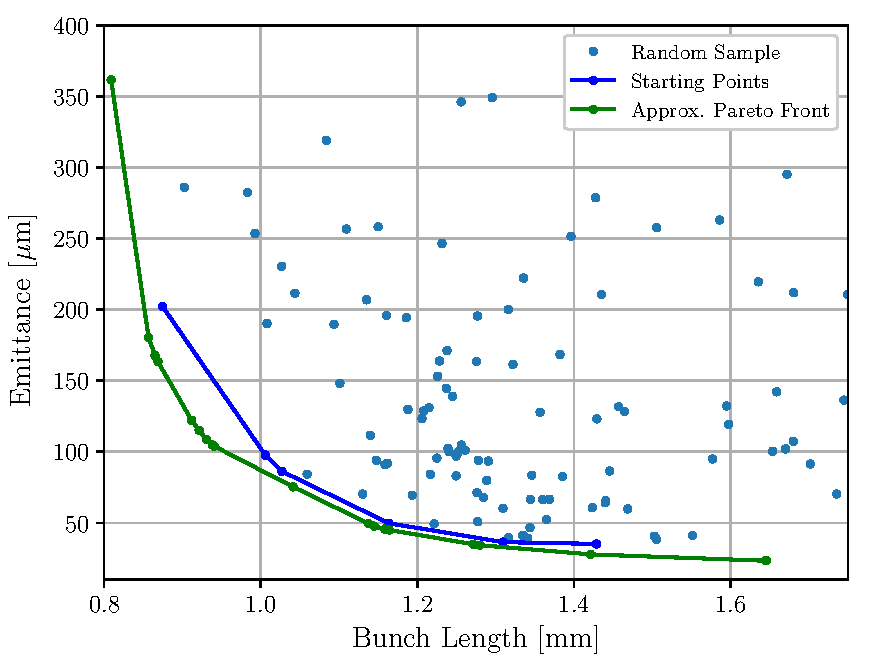
\includegraphics[width=0.98\textwidth]{images/THPAB155f1}
		\caption{Random sample results, starting sample points, and resulting approximate Pareto front for the linac at \SI{40}{nC}. The Pareto front is the result of all BOBYQA evaluations.}
		\label{fig:pareto}
	\end{center}
\end{figure}
This can be aided by examining a Pareto front: the set of parameters 
for which no other point exists that is better with respect to both objectives~\cite{ehrgott2006multicriteria}.
In Figure~\ref{fig:pareto}, blue dots show the emittance and bunch length for the
evaluated random sample. The sample points for which no other point has better
emittance and bunch length are connected with a blue line. BOBYQA was started
from these points, as described above, producing the green approximate Pareto front. 


The number of simulation evaluations needed to obtain convergence
in the BOBYQA runs varied from a minimum of 107 evaluations to a maximum of 208 
evaluations. In order to generate the Pareto front in
Figure~\ref{fig:pareto}, a total of 2,492 simulation evaluations were completed.
Most simulation evaluations took approximately 7 minutes, using 16 cores and 100,000 particles. These numbers are driven by the amount of time OPAL-T needs to simulate the beam line. 

The best-found objective value through each BOBYQA run is shown in Figure~\ref{fig:iterations}. 
Weight 0.0 and 1.0 are negative due to the scaling in Equation~(\ref{eq:scale}). While the weights, $w$, are always nonnegative, 
$\bar{\epsilon}_x (v,z_1)$ or $\bar{\sigma}_z(v,z_1)$ will be negative if BOBYQA finds a point with a value of 
$\epsilon_x(v,z_1)$ or $\sigma_z(v,z_1)$ that is less than $\epsilon_{\min}$ or $\sigma_{\min}$ from the initial sample. 
\begin{figure}[h]
	\captionsetup{width=0.98\linewidth}
	\begin{center}
		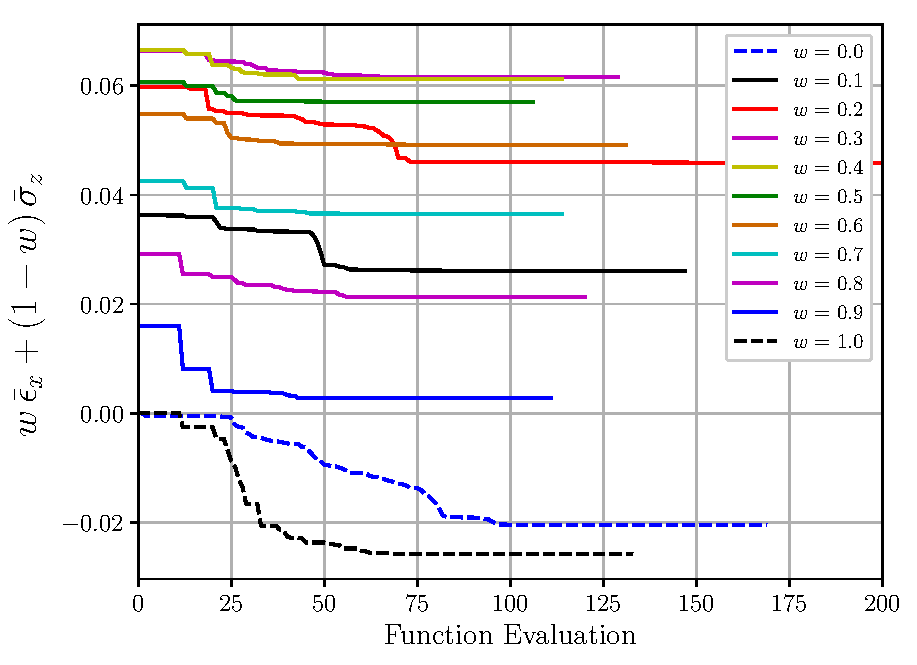
\includegraphics[width=0.98\textwidth]{images/THPAB155f2}
		\caption{\label{fig:iterations}Minimum observed objective function values during eleven BOBYQA runs at \SI{40}{nC}.}
	\end{center}
\end{figure}

We note that seven of the BOBYQA runs converged to emittance values
between \SI{20}{\mu m} and \SI{50}{\mu m}, which is shown in Figure~\ref{fig:trade} 
along with gun phase and bunch length for each of the 11
optimized points. We annotate Figure~\ref{fig:trade} with $T$ because that parameter 
shows strong correlation with the gun phase. Other optimized parameters such as the laser radius were found to stay within a 
narrow range (\SIrange{10}{16}{mm}).  
\begin{figure}[h]
	\captionsetup{width=0.98\linewidth}
	\begin{center}
		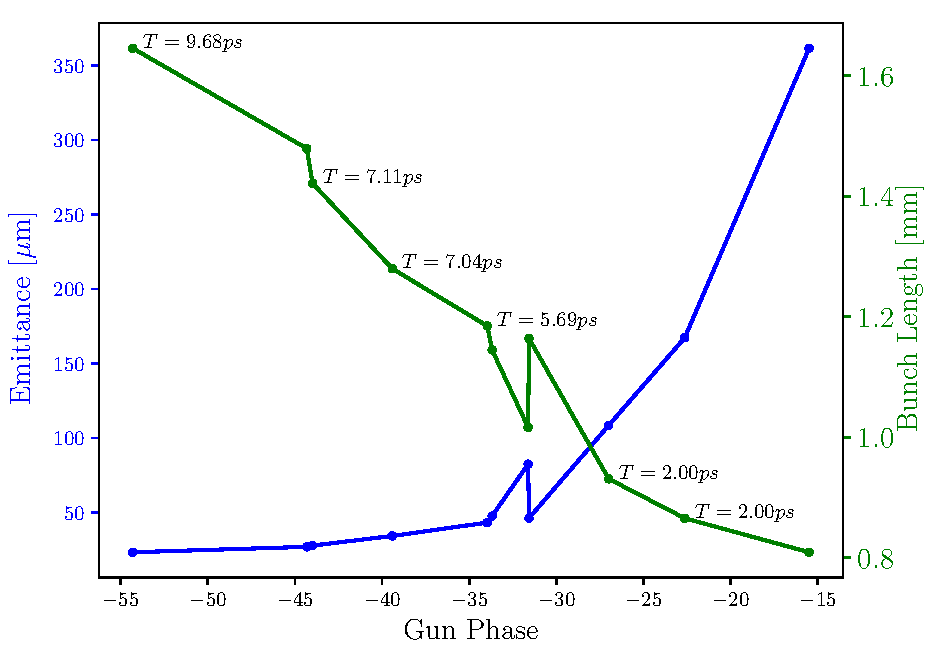
\includegraphics[width=0.98\textwidth]{images/THPAB155f3}
		\caption{\label{fig:trade}Bunch length and emittance vs.~gun phase at each optimized point in the Pareto front for the linac at \SI{40}{nC}. The phase of the max energy gain is 0$^{\circ}$.}
	\end{center}
\end{figure}


The optimized linac phases maximize energy gain while minimizing the energy spread.
The energy spread of the beam exiting the gun depends strongly on $\phi_g$.
There are three distinct regions where the optimized points had similar gun phases 
(less than $\pm10^{\circ}$) which resulted in nearly identical linac phases. For example:  
all six phases, $\phi_L$, varied by less than $10^{\circ}$ for $w \in \left\{ 0, 0.1\right\}$,
less than $5^{\circ}$ for $w \in \left\{ 0.4, 0.5, 0.6\right\}$, 
and less than $10^{\circ}$ for $w \in \left\{ 0.7, 0.8, 0.9\right\}$.
This indicates optimized linac phases may benefit a range of gun settings during operation. 


\Subsection{Lessons Learned from BOBYQA Work}
\nrnote{conclusion from paper... add some?}
% ----------------------------------------------------
Using an AWA beam line as the simulation model, we used the BOBYQA algorithm 
to optimize the emittance produced by the gun at \SI{1}{nC}.
Using the same algorithm, we performed a multiobjective analysis for the linac at \SI{40}{nC}. 
A Pareto front comparing the trade-off between bunch length and emittance was generated for the linac. 
In total, only 2,492 simulation evaluations were needed to produce the approximate Pareto front.
From this work a few key take aways are clear. First, larger laser radius
is uniformly better for high charge. i.e large radius helps lower emittance.
The second clear results is alternating the phases in the linac can control 
the energy spread created by the gun, i.e. running off crest in the linac 
can reduce the energy spread significantly.

%%%%%%%%%%%%%%%%%%%%%%%%%%%%%%%%%%%%%%%%%%%%%%%%%%%%%%%%%%%%%%%%%%%%%%%%%%%%%%%%
%%%%%%%%%%%%%%%%%%%%%%%%%%%%%%%%%%%%%%%%%%%%%%%%%%%%%%%%%%%%%%%%%%%%%%%%%%%%%%%%
\Section{OPAL and the Genetic Algorithm: NSGA-II} \label{sec:ga}
%%%%%%%%%%%%%%%%%%%%%%%%%%%%%%%%%%%%%%%%%%%%%%%%%%%%%%%%%%%%%%%%%%%%%%%%%%%%%%%%
%%%%%%%%%%%%%%%%%%%%%%%%%%%%%%%%%%%%%%%%%%%%%%%%%%%%%%%%%%%%%%%%%%%%%%%%%%%%%%%%
Next, work began on designing the TBA experimental area. 
Initial probes into this problem were done using the genetic algorithm
implemented in OPAL-T~\cite{optpilot}.

\lsnote{\Section{Summary}}\\
\lsnote{Reiterate the flow of the chapter and the main results of your work.}
